\documentclass{article}

\usepackage[T1]{fontenc}
\usepackage{siunitx}
\usepackage[polish]{babel}
\usepackage[utf8]{inputenc}
\usepackage{float}
\usepackage{graphicx}
\usepackage{amsmath}
\usepackage{siunitx}
\usepackage{longtable}
\usepackage{pdfpages} 
\oddsidemargin 0pt
\evensidemargin 0pt
\marginparwidth 40pt
\marginparsep 10pt
\topmargin -20pt
\headsep 10pt
\textheight 8.7in
\textwidth 6.65in
\linespread{1.2}

\title{Sprawozdanie z Laboratorium 6.}
\author{Piotr Lewandowski \and Dymitr Lubczyk \and Krzysztof Tabeau }
\date{\today}
\begin{document}
\maketitle
\subsection{Informacje}
\begin{tabular}{|l|l|}
\hline
Autorzy             & Dymitr Lubczyk                    \\
                    & Krzysztof Tabeau                  \\
                    & Piotr Lewandowski                 \\
Wydział             & Matematyki i Nauk Informacyjnych  \\
Numer Zespołu       & 19                                \\
Data laboratorium   & 17:15 15.06.2020                  \\
Numer laboratorium  & 6                                 \\
Prowadzący          & dr Janusz Oleniacz                \\
\hline
\end{tabular}

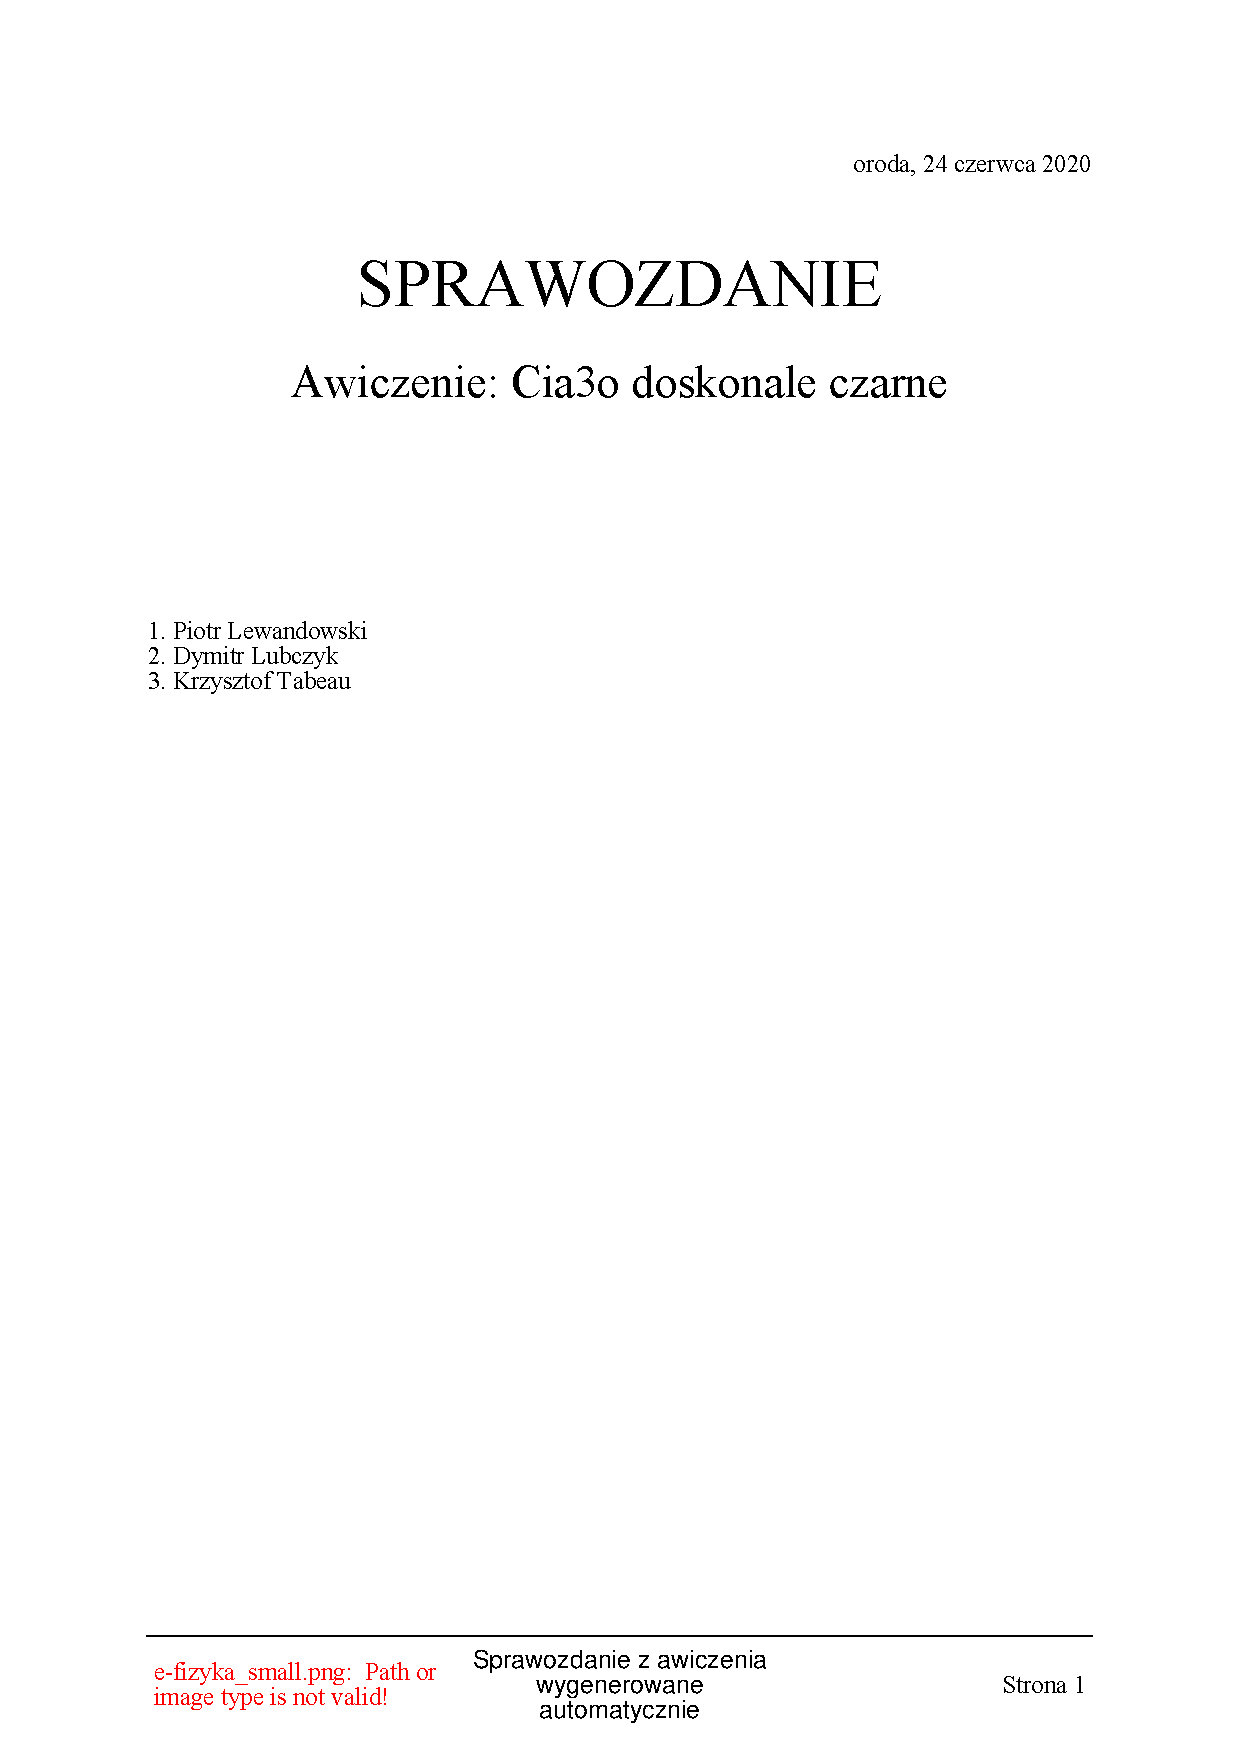
\includepdf[page=-]{Sprawozdanie}

\clearpage
\section{Generowanie widm, liczenie promieni słońca}
\subsection{Wyniki}
Poniżej przedstawione są wyniki rozkładu promieniowania dla ciała doskonale czarnego przy określonych temperaturach:
\begin{figure}[H]
    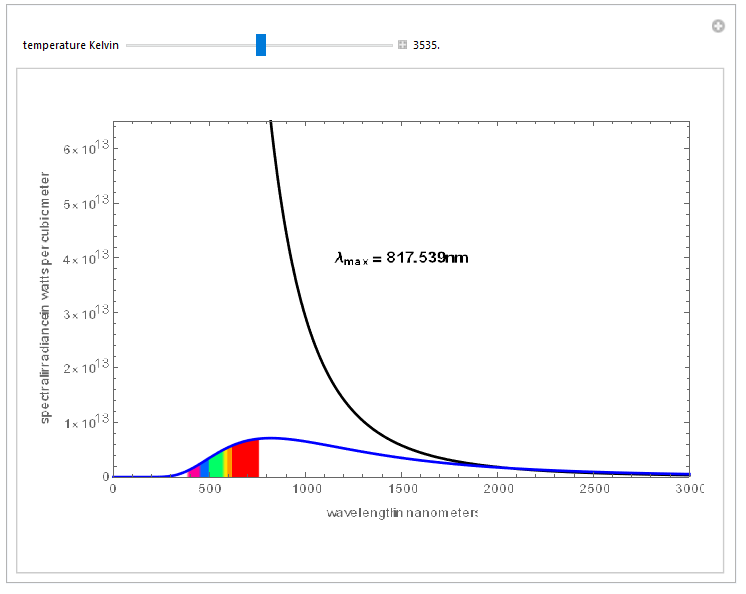
\includegraphics[width=\textwidth]{DL2.1.PNG}
    \caption{3535K}
\end{figure}
\begin{figure}[H]
    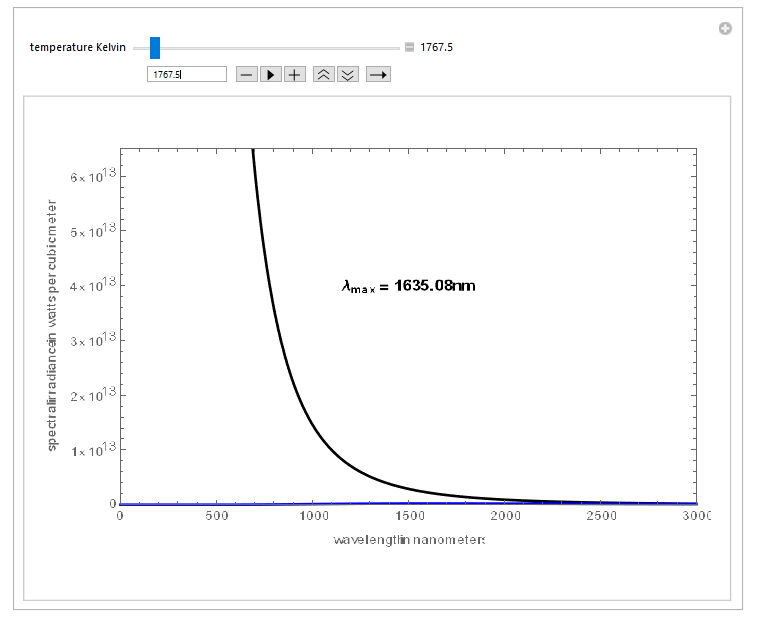
\includegraphics[width=\textwidth]{DL2.2.PNG}
    \caption{1767K}
\end{figure}
\begin{figure}[H]
    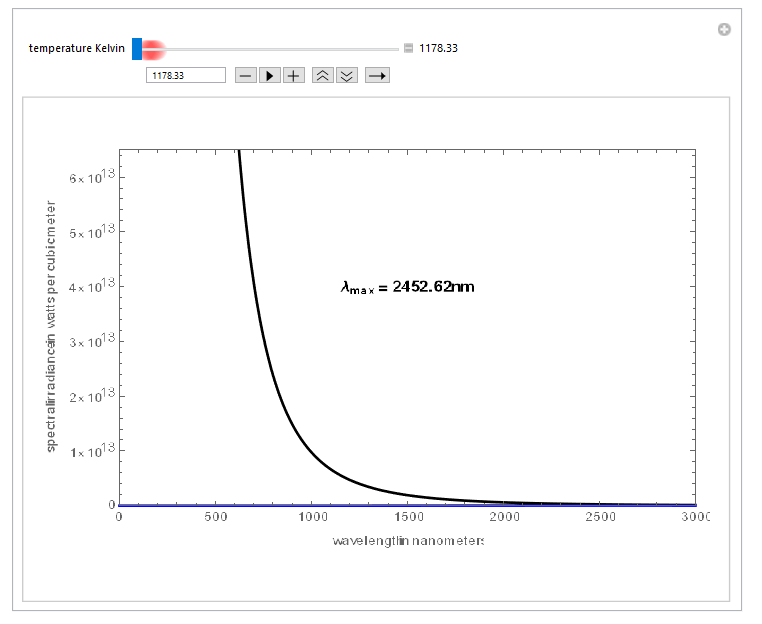
\includegraphics[width=\textwidth]{DL2.3.PNG}
    \caption{1178K}
\end{figure}
\begin{figure}[H]
    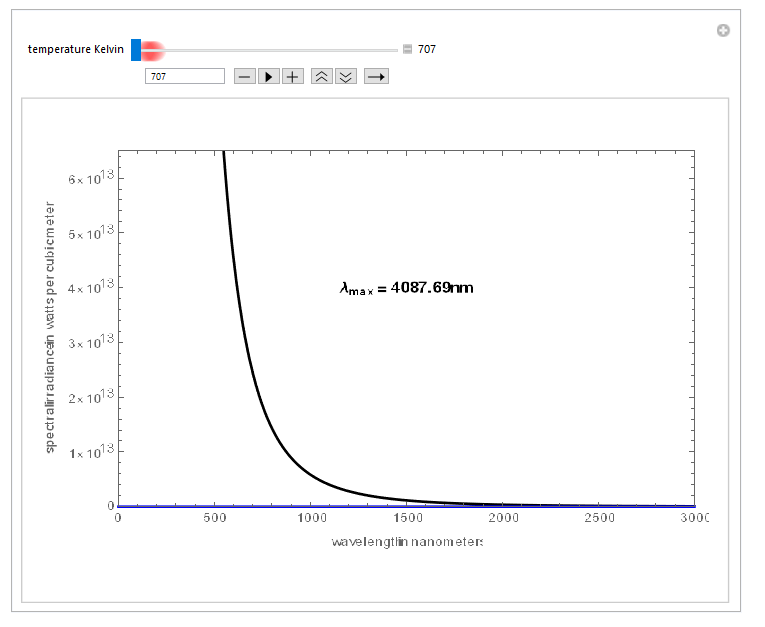
\includegraphics[width=\textwidth]{DL2.4.PNG}
    \caption{707K}
\end{figure}
\begin{figure}[H]
    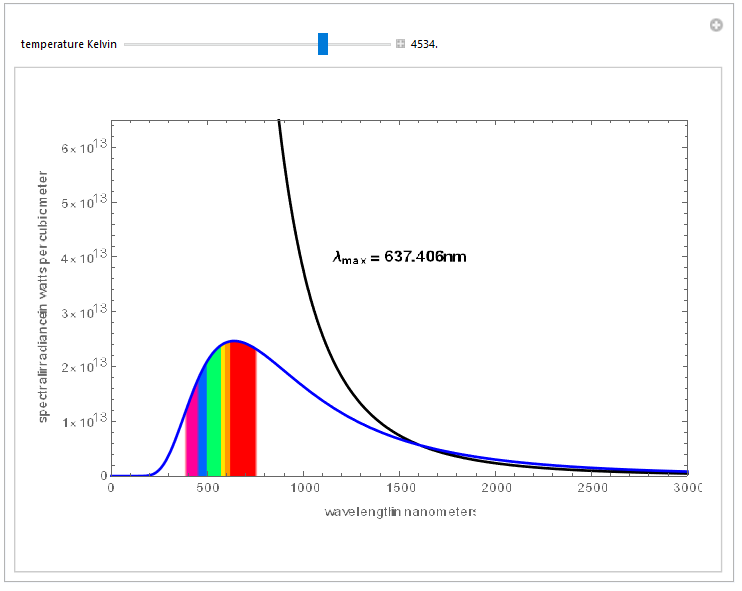
\includegraphics[width=\textwidth]{PL2.1.PNG}
    \caption{4534K}
\end{figure}
\begin{figure}[H]
    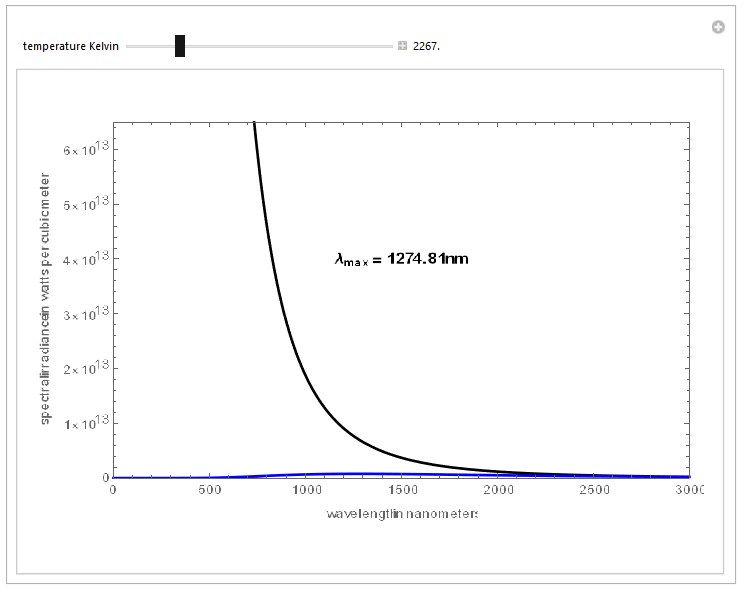
\includegraphics[width=\textwidth]{PL2.2.PNG}
    \caption{2267K}
\end{figure}
\begin{figure}[H]
    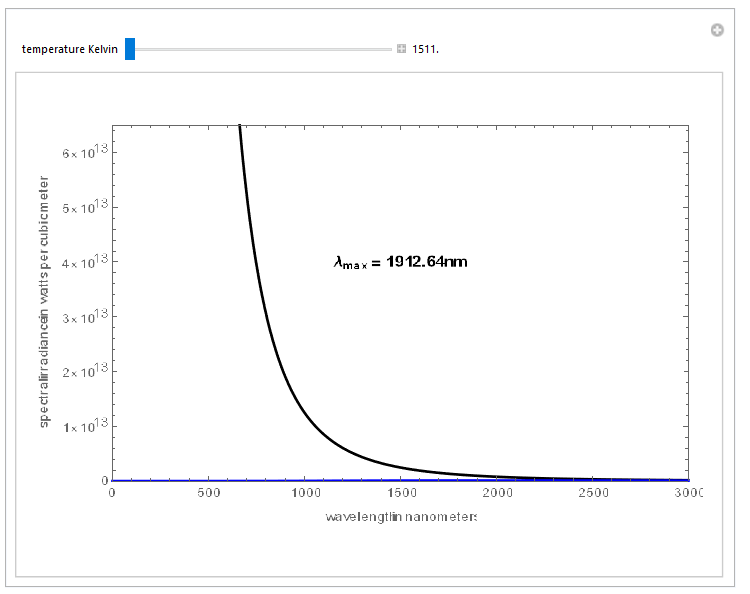
\includegraphics[width=\textwidth]{PL2.3.PNG}
    \caption{1511K}
\end{figure}
\begin{figure}[H]
    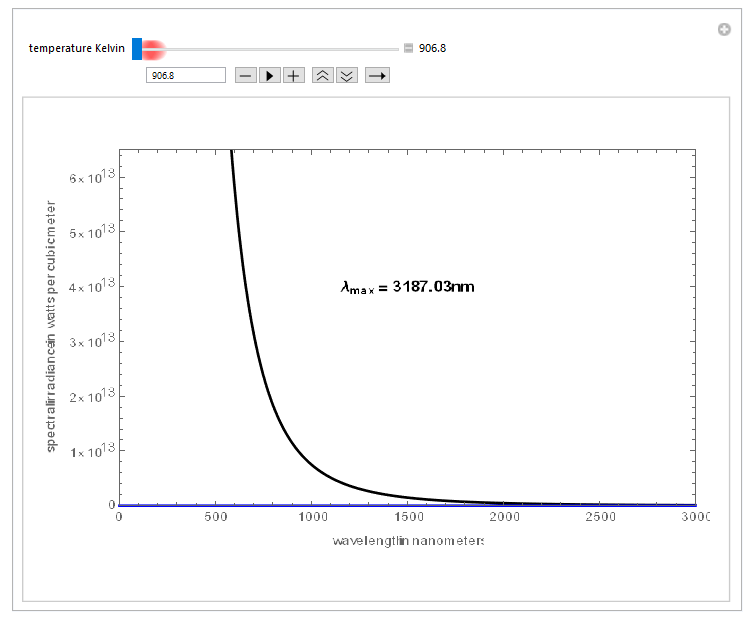
\includegraphics[width=\textwidth]{PL2.4.PNG}
    \caption{906K}
\end{figure}
\begin{figure}[H]
    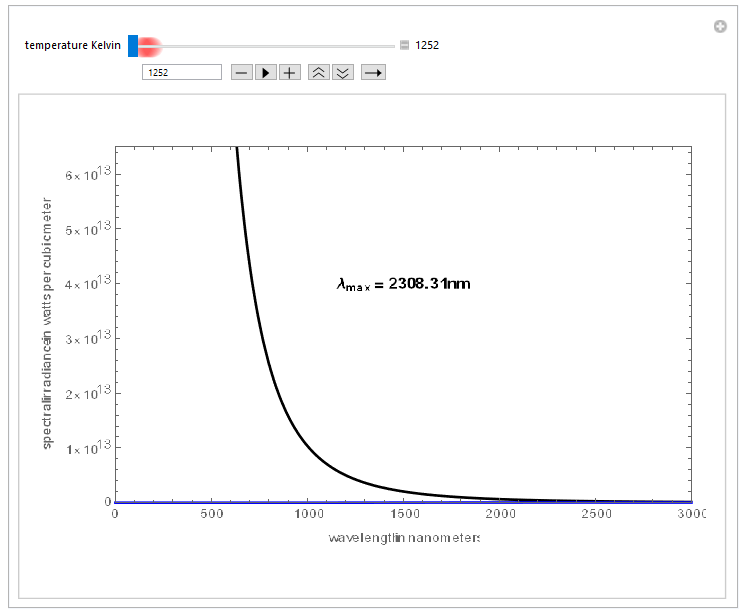
\includegraphics[width=\textwidth]{KT2.2.PNG}
    \caption{1252K}
\end{figure}
\begin{figure}[H]
    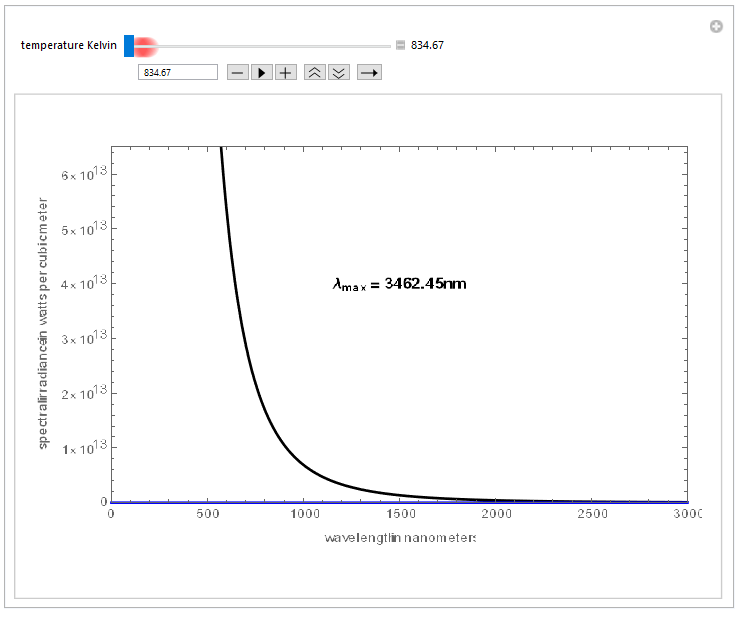
\includegraphics[width=\textwidth]{KT2.3.PNG}
    \caption{834K}
\end{figure}
\begin{figure}[H]
    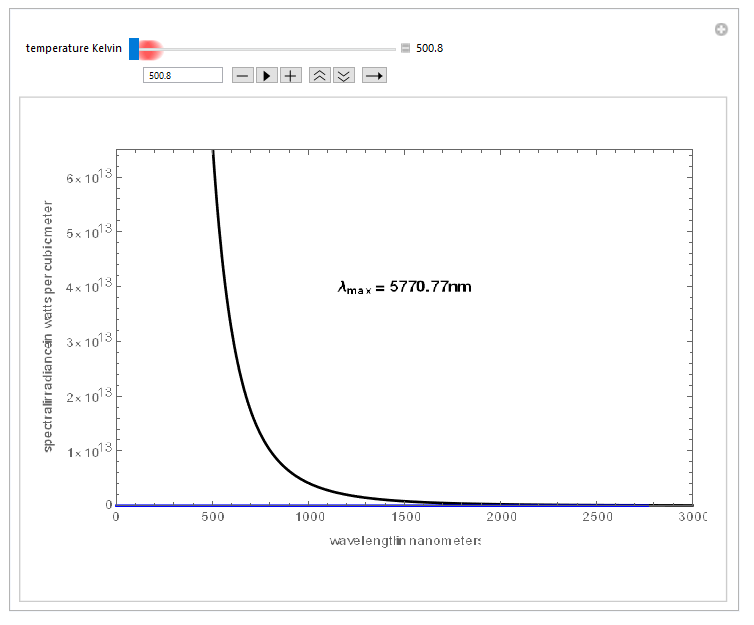
\includegraphics[width=\textwidth]{KT2.4.PNG}
    \caption{500K}
\end{figure}
\clearpage
\subsection{Wnioski}
Poniżej widzimy tabelkę przestawiającą obliczone z prawa
\begin{table}[h!]
\centering
\begin{tabular}{|l|l|l|l|}
\hline
$ \lambda_{max}[nm]$ & T[K] & $T*\lambda_{max}$ & $r[km]$ \\ \hline
1154 & 2504 & 2.89E+06 & 3,707,727 \\
817 & 3535 & 2.89E+06 & 1,860,363 \\
637 & 4534 & 2.89E+06 & 1,130,872 \\
2308 & 1252 & 2.89E+06 & 14,830,909 \\
1635 & 1767.5 & 2.89E+06 & 7,441,450 \\
1274 & 2267 & 2.89E+06 & 4,523,487 \\
3462 & 834 & 2.89E+06 & 33,369,278 \\
2452 & 1178 & 2.89E+06 & 16,743,357 \\
1912 & 1511 & 2.89E+06 & 10,177,891 \\
5770 & 500 & 2.89E+06 & 92,693,179 \\
4087 & 707 & 2.89E+06 & 46,509,063 \\
3187 & 906 & 2.89E+06 & 28,271,796 \\
\hline
\end{tabular}
\caption{Wyniki dla światła zielonego}
\end{table}
Patrząc na trzecią kolumnę widzimy, że iloczyn T i $\lambda_{max}$ jest stały co więcej jest on równy stałej Stefana-Boltzmanna pomnożonej przez $10^9$ wynika to z tego, że długość fali zapisana jest w nm. Obserwacja ta pozwala nam przypuszczać, ze prawo Stefana-Boltzmanna jest prawdziwe. Przechodząc do 4 kolumny widzimy promień jaki musiałoby mieć słońce, aby mieć tę samą moc, przy zależeniu temperatury z kolumny 2, jak nieciężko się domyślić wraz ze spadkiem temperatury, promień rośnie.
\end{document}



















